\section{An\'alisis}

\subsection{Descripci\'on}

Este prototipo permite la visualizaci\'on del funcionamiento de la API de an\'alisis mediante un sistema de mensajer\'ia.

\subsection{Objetivo}
Generar un sistema de mensajer\'ia sobre el cual el funcionamiento de la API de an\'alisis ser\'a visualizado. 

\subsection{Caracter\'isticas}

\begin{description}
\item[FEAT1] El usuario puede registrarse al sistema.
\item[FEAT2] El usuario puede ingresar al sistema.
\item[FEAT3] El usuario puede visualizar su lista de contactos.
\item[FEAT4] El usuario puede agregar a otros usuarios a su lista de contactos.
\item[FEAT5] El usuario puede conversar con otros usuarios.
\item[FEAT6] El usuario puede vizualizar si las conversaciones en las cuales ha participado son peligrosas.

\end{description}

\subsection{Restricciones}
\begin{itemize}
\item Prototipo desarrollado con el framework Django 1.7.
\item Desarrollado con python 2.7.
\end{itemize}

\subsection{Casos de uso}

\section{Modelo de casos de uso del sistema de mensajer\'ia}

El siguiente diagrama de casos de uso muestra las acciones que el usuario podr\'a realizar dentro del sistema de mensajer\'ia. El usuario, llamado Contacto, ser\'a capaz de realizar las siguientes actividades:
\begin{itemize}
	\item Registrar de contacto
\item Iniciar sesi\'on
\item Agregar contacto a una lista
\item Enviar mensaje
\item Cerrar sesi\'on
\end{itemize}
	\begin{figure}[htbp!]
		\centering
			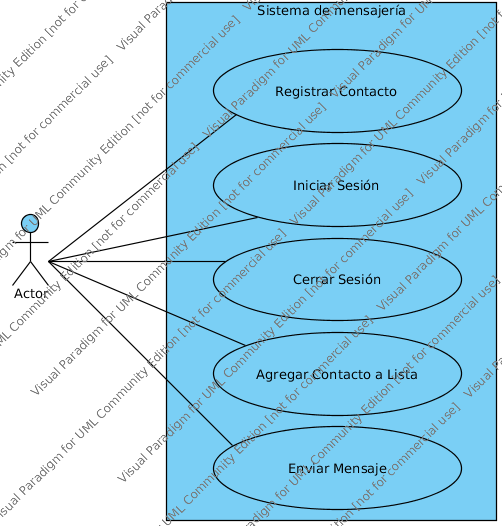
\includegraphics[width=0.8\textwidth]{images/Diagramas/dcasosdeuso}
		\caption{Diagrama de Casos de Uso del sistema de mensajer\'ia.}
	\end{figure}
	
	
	\pagebreak
